\chapter{Methods}
\label{chap:method}                                   
\setstretch{1.5}                                       
\section{Robot Task}                                   
\label{sec: usecase}                                   
A pick and place application was created to test the collision avoidance system. The pick and place task is an endless loop, where the robot uses its vacuum gripper to move two wooden shingles from one side of the table to the other side and then back again. Figure \ref{fig:robotask} illustrates the robot movements with arrows pointing in the direction of the robot goal position.
                                                       
\begin{figure}[H]                                      
	\centering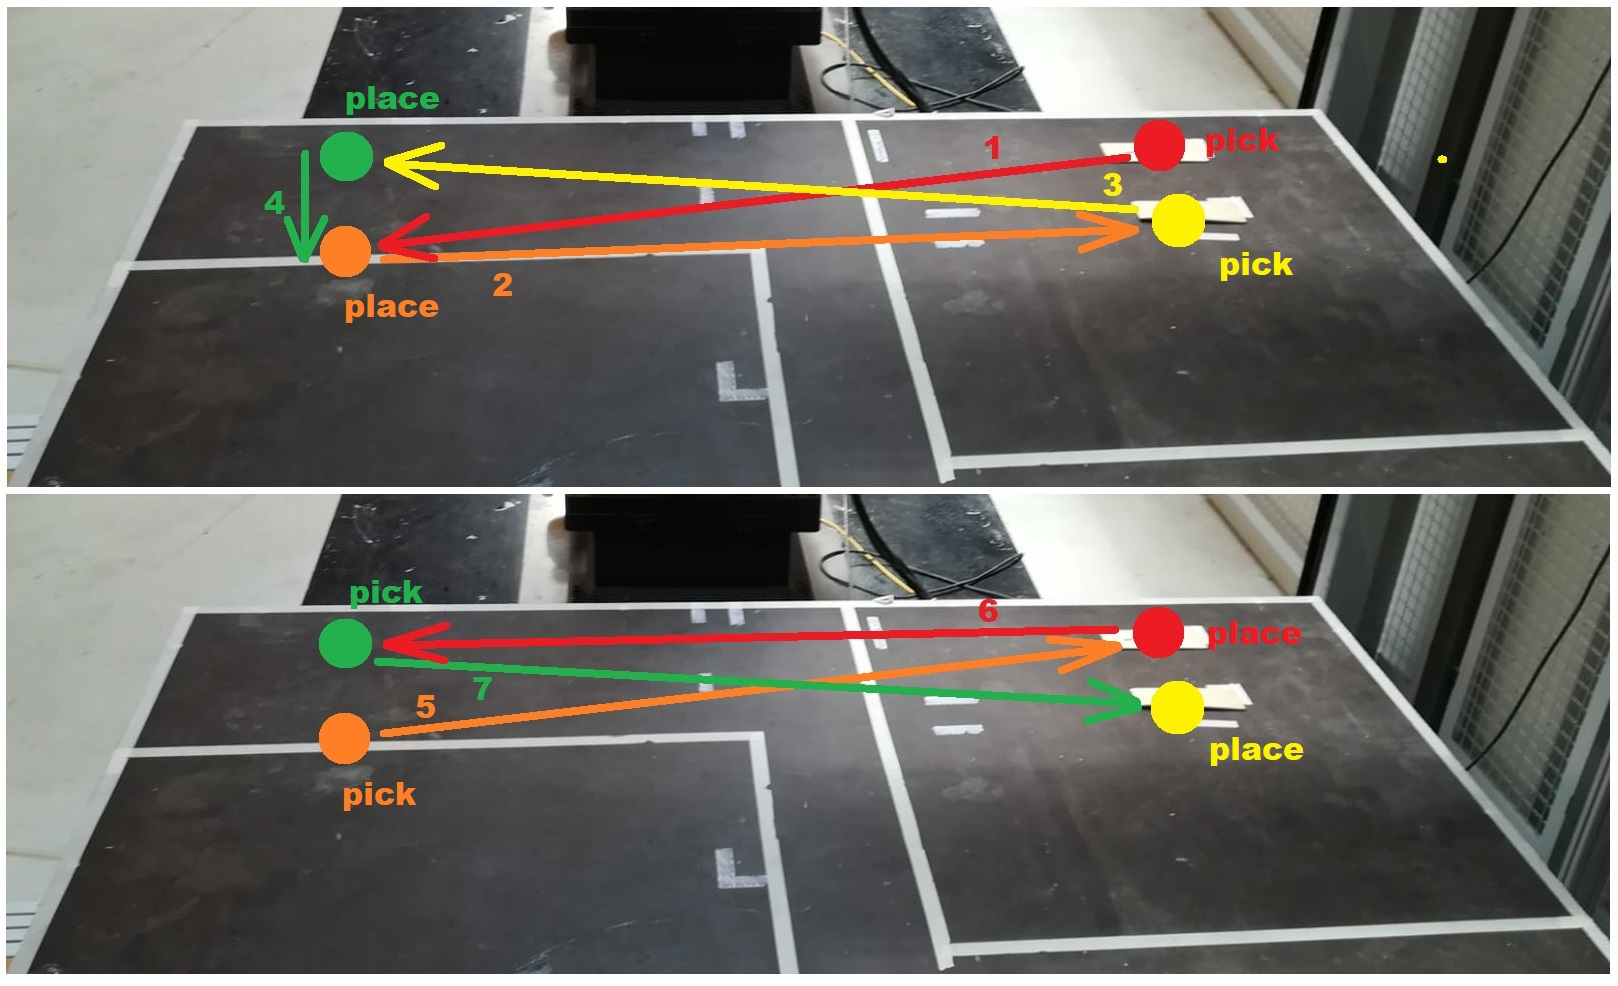
\includegraphics[scale=0.38]{images/robot_task.jpeg}		
	\caption{Robot task visualised.}   
	\label{fig:robotask}                    
\end{figure}                                           
\section{Robot communication}                          
\label{sec:robcom}                                     
As a first task, the communication between the collision avoidance system and the robot has to be established. A sequential communication approach was chosen since it provides a stable functionality and additional control over the process. The communication on the system side is run by a single TP program calling two KAREL programs, one for reading current robot positions of the robot, and one for writing go-to positions where the robot has to move to and and additional TP program to actually move the robot. The communication on the system side is provided by two functions written in C++. The sequential communication is run on the robot and uses flags in each of the KAREL and TP programs to trigger a certain function call. Listing \ref{lst:robcom} shows the TP program which runs the sequential communication TP program. The user frame and the tool are defined at program start. The position register is initialized with the correct type and the flags are set in their default value. The default value is set to be ready to send the current robot position to the collision avoidance system.
\begin{figure}[H]
\begin{lstlisting}[frame = single, caption={TP Program which enables the sequential communication.}, captionpos=b, label={lst:robcom}]
1:  UFRAME_NUM=8 ;
2:  UTOOL_NUM=3 ;
3:  PR[90]=LPOS    ;
4:  R[200]=(1) ;
5:  R[199]=(0) ;
6:  LBL[100] ;
7:  IF (R[200]=1 AND R[199]=0) THEN ;
8:  	CALL TEST_READ_C    ;
9:  ENDIF ;
10: IF (R[200]=0 AND R[199]=1) THEN ;
11:  	CALL TEST_WRITE_C    ;
12: ENDIF ;
13: IF (R[200]=0 AND R[199]=0) THEN ;
14:  	CALL ROS_MOVESM    ;
15: ENDIF ;
16: JMP LBL[100] ;
\end{lstlisting}
\end{figure} 				                                              
\subsection{Send and Read Robot Positions}   
          
\label{subsec:sendread}                                
\lstset{language=Pascal,
	basicstyle=\ttfamily,
	numbers=left,
	stepnumber=1,
	keywordstyle=\color{blue},
	stringstyle=\color{red},
	commentstyle=\color{green},
	morecomment=[l][\color{magenta}]{\#}
}          
The KAREL programs start with a header specifying different items like program name and environment settings. The KAREL programs of this project start both with almost exactly the same header part, only differentiating in the program name. Listing \ref{lst:karelhead} shows the file header of the read program.
\begin{figure}[H]
\begin{lstlisting}[frame = single, caption={KAREL header of the "read robot positions" function}, captionpos=b, label={lst:karelhead}]  
PROGRAM test_read_c
%STACKSIZE = 4000
%NOLOCKGROUP
%NOPAUSE=ERROR+COMMAND+TPENABLE
%ENVIRONMENT uif
%ENVIRONMENT sysdef
%ENVIRONMENT memo
%ENVIRONMENT kclop
%ENVIRONMENT bynam
%ENVIRONMENT fdev
%ENVIRONMENT flbt
%ENVIRONMENT REGOPE
%INCLUDE klevccdf
%INCLUDE klevkeys
%INCLUDE klevkmsk
\end{lstlisting}
\end{figure} 
\begin{tabbing}
	xxxxxxxxxxxxxxxxxxxxxxxxxxxx\=xxxxxxxxxxxxxxxxxxxxxxxxxxxxxxxxxxxxxxxxxxxxxxxxxxxxxxxxxxxxxxxxxx \kill
	PROGRAM:	\> Specifies the program name, max. 12 characters.	\\	
	\%STACKSIZE = n:		\>  Specifies the stack size in long words. \\				
	\%NOPAUSE = option:	\> Specifies a set of conditions which will  be prevented from pausing\\
						\>  the program. 		\\							% insert names
	\%ENVIRONMENT filename:	\> Used by the off-line translator to specify that a particular environment\\
					\> file should be loaded. 				\\	
	\%INCLUDE filename:		\>  Specifies files to insert into a program at translation time. 				\\							% insert names
	
\end{tabbing}
Listin \ref{lst:karelseq1} shows the second part of the KAREL program which specifies variables, which will be used during program execution.
\begin{figure}[H]
\begin{lstlisting}[frame = single, caption={KAREL variable definitions}, captionpos=b, label={lst:karelseq1}]
VAR
file_var   : FILE
STATUS  : INTEGER
entry   : INTEGER
cur_pos: XYZWPR		-- Robot position
-- REAL Array to convert to robot position
c_real_array : ARRAY[6] OF REAL  
indx   : INTEGER    --for counter

CONST
-- POS Register Number wich will be used to store the current
   robot position
MOVE_PREG = 90
-- Flags to indicate which step is next. used in ROB195_COM.ls
WRITE_FLAG = 199
READ_FLAG = 200
\end{lstlisting}
\end{figure} 
After the variable definitions the actual program sequence starts by setting up the server port and opening the file variable to write the current robot position as shown in listing \ref{lst:karelconnect}. The port 59004 is used for the read command and port 59003 is used for the write command.
\begin{figure}[H]
\begin{lstlisting}[frame = single, caption={KAREL start connection to client.}, captionpos=b, label={lst:karelconnect}]
BEGIN
indx = 1	
FORCE_SPMENU(TP_PANEL,SPI_TPUSER,1)
WRITE TPDISPLAY (CHR(128),CHR(137))
SET_FILE_ATR(file_var, ATR_IA)
-- set the server port before doing a connect
SET_VAR(entry, '*SYSTEM*',
  '$HOSTS_CFG[3].$SERVER_PORT',59004,STATUS)
WRITE TPDISPLAY('Connecting..',CR)
MSG_CONNECT('S3:',STATUS) -- connecting to system
WRITE TPDISPLAY(' CONNECT STATUS = ',STATUS,CR)
IF STATUS = 0 THEN -- checks connection status
-- Open S3:
	WRITE TPDISPLAY('Opening',CR)
	OPEN FILE file_var ('rw','S3:')
	STATUS = IO_STATUS(file_var)
	WRITE TPDISPLAY(STATUS,CR)
\end{lstlisting}
\end{figure}

When the connection is successful, the current robot position is written to the cur\_pos variable using the CURPOS built-in function, which returns the XYZ coordinates as well as the WPR angles. The current position needs then to be written into the real array in order to write it to the file variable and send it to the system. 
\begin{figure}[H]
\begin{lstlisting}[frame = single, caption={KAREL read current robot position and prepare the data for sending.}, captionpos=b, label={lst:karelvarprep}]
 IF STATUS = 0 THEN
-- write an integer
	cur_pos = CURPOS(0,0)
	
	c_real_array[1] = cur_pos.X
	c_real_array[2] = cur_pos.Y
	c_real_array[3] = cur_pos.Z
	c_real_array[4] = cur_pos.W
	c_real_array[5] = cur_pos.P
	c_real_array[6] = cur_pos.R
\end{lstlisting}
\end{figure}
After preparing the position data, it is sent using a for statement to loop through the REAL array and send each coordinate. Afterwards the file variable is closed and the client is disconnected. The flags are set in order to start the writing step.
\begin{figure}[H]
\begin{lstlisting}[frame = single, caption={KAREL sending position data and closing connection.}, captionpos=b, label={lst:karelread}]
		FOR indx = 1 TO 6 DO
			WRITE file_var(c_real_array[indx], CR)
		ENDFOR
		CLOSE FILE file_var
	ENDIF
	WRITE TPDISPLAY('Disconnecting..',CR)
	MSG_DISCO('S3:',STATUS)
	WRITE TPDISPLAY('Done.',CR)
	SET_INT_REG(WRITE_FLAG, 1, STATUS)
	SET_INT_REG(READ_FLAG, 0, STATUS)
ENDIF
END test_read_c
\end{lstlisting}
\end{figure}
The write command is build in the same manner but reverses the steps. This means the position is written into the real array and then converted to the position variable, which is then stored in the position register of the robot controller. The code can be found in the appendix \ref{app:karelread} on page \pageref{app:karelread}. The program for the read and write functions is based on the socket communication example from the KAREL reference manual for the R-30iA controller \cite{refman}.

The systems uses two C++ functions to either read position data from the robot or write goal positions for the robot. Listing \ref{lst:cppread1} shows the first part of the read function, where the host address and port are set up.

\lstset{language=C++,
	numbers=left,
	stepnumber=1,
	basicstyle=\ttfamily,
	keywordstyle=\color{blue},
	stringstyle=\color{red},
	commentstyle=\color{green},
	morecomment=[l][\color{magenta}]{\#}
}
\begin{figure}[H]
\begin{lstlisting}[frame = single, caption={C++ Set up host adress and port.}, captionpos=b, label={lst:cppread1}]
float *connectReadCartesian (float *current_cartesian_pos){
// READ SETUP
	int sockfd;
	struct sockaddr_in serv_addr_read;
	bzero((char *) &serv_addr_read, sizeof(serv_addr_read));
	serv_addr_read.sin_family = AF_INET;
	serv_addr_read.sin_addr.s_addr = inet_addr(SERV_HOST_ADDR);
	serv_addr_read.sin_port = htons(SERV_TCP_PORT_READ);
\end{lstlisting}
\end{figure}
Listing \ref{lst:cppread2} shows the second part of the read function, where the client connects to the host. When the connection is successful, the \emph{readPos()} function is called, which reads the six parts of the robot position, each character separately.
\begin{figure}[H]
\begin{lstlisting}[frame = single, caption={C++ connect to host and read current robot position.}, captionpos=b, label={lst:cppread2}]
// READ POS

	if((sockfd = socket(AF_INET, SOCK_STREAM,0)) < 0){
	  printf("Client: Can't Open Stream Socket\n");
	}
	printf("Client: Connecting to READ server...\n");
	  while(connect(sockfd,(struct sockaddr *) ...
		   &serv_addr_read, sizeof(serv_addr_read))<0){
	  printf("Client: Can't Connect to the READ server\r");
	}

	printf("Client: Connected!\n");
	current_cartesian_pos = readPos(sockfd);

	return current_cartesian_pos;
}
\end{lstlisting}
\end{figure}
Writing goal positions for the robot has the same functionality as reading the positions, but again in reverse. Each character of the six coordinates separately. The code for the write function can be found in appendix \ref{app:com_func.cpp}.
                       
\subsection{Robot movements}
\label{subsec:robmove}

\lstset{language=Pascal,
	basicstyle=\ttfamily,
	numbers=left,
	stepnumber=1,
	keywordstyle=\color{blue},
	stringstyle=\color{red},
	commentstyle=\color{green},
	morecomment=[l][\color{magenta}]{\#}
}       
The robot movements are done by using the linear movement function provided by the built-in library of Fanucs TP programming language. Listing \ref{lst:robmove} shows the TP program, which moves the robot to the specified position in the position register \#90. First it defines the tool and the frame in which the robot should move. Then the linear movement is specified by its end position, speed and if the point is a fixed point or a via point. FINE states that the point is a fixed point which has to be exactly reached. The flags R[200] and R[199] are used to trigger the next step of the sequence of the communication.
\begin{figure}[H]
\begin{lstlisting}[frame = single, caption={TP Move the robot the the specified position.}, captionpos=b, label={lst:robmove}]
1:  UTOOL_NUM=3 ;
2:  UFRAME_NUM=8 ;
3:L PR[90] 250mm/sec FINE ;
5:  R[200]=(1) ;
6:  R[199]=(0) ;
\end{lstlisting}
\end{figure}
\subsection{Gripping commands}
\label{subsec:gripcom}
\lstset{language=[5.3]LUA,
	numbers=left,
	stepnumber=1,
	basicstyle=\ttfamily,
	keywordstyle=\color{blue},
	stringstyle=\color{red},
	commentstyle=\color{green},
	morecomment=[l][\color{magenta}]{\#}
}
Usually the gripping commands would be executed using fieldbus communication. However, currently no working fieldbus communication is available on the robot. 

In order to have a very simple communication to send gripping commands, two simple LUA scripts (listing \ref{lst:telnet}) were written, each connecting to the robot controller over telnet writing a specified value to a digital out of the robot, that activates the gripper.
\begin{figure}[H]
\begin{lstlisting}[frame = single, caption={LUA Script for telnet connection.}, captionpos=b, label={lst:telnet}]  
  --set up telnet conn
local ip = '147.87.144.251';
local port = 23; -- TELNET
local sock = require('socket');
local serv, err = sock.connect(ip, port);
local action = 0 -- actual gripping command
--actuation
serv:send('LOGIN\r');
sock.sleep(0.15);
serv:send('PASSWORD\r');
sock.sleep(0.15);
serv:send('set port rdo[7]='.. action.. '\r');
sock.sleep(0.25);
serv:close();
\end{lstlisting}
\end{figure}
The two LUA scripts only differ in the value of the variable "local action" on listing \ref{lst:telnet} on line six. A "0" is used to disable the vacuum of the gripper, and a "1" is used to enable the gripper vacuum. In order to improve code readability, two C++ functions were implemented named gripperOn (listing \ref{lst:gripON})/ gripperOff (listing \ref{lst:gripOFF}) located in the com\_func.cpp file.

\lstset{language=C++,
	numbers=left,
	stepnumber=1,
	basicstyle=\ttfamily,
	keywordstyle=\color{blue},
	stringstyle=\color{red},
	commentstyle=\color{green},
	morecomment=[l][\color{magenta}]{\#}
}
\begin{figure}[H]
\begin{lstlisting}[frame = single, caption={gripperOn function}, captionpos=b, label={lst:gripON}]  
void gripperOn (void){
	system("lua5.3 ../Rob195/1.txt");
}
\end{lstlisting}
\end{figure}
\begin{figure}[H]
\begin{lstlisting}[frame = single, caption={gripperOff function}, captionpos=b, label={lst:gripOFF}]  
void gripperOff (void){
	system("lua5.3 ../Rob195/0.txt");
}
\end{lstlisting}
\end{figure}
\section{Data gathering, workspace monitoring}
\label{sec:datagather}
\subsection{Camera positioning}
\label{subsec:campos}
The original camera design did not allow to mount the camera with screws in a fixed position as seen in figure \ref{fig:asus} in section \ref{subsec:asus}. In order to be able to do so, a fixture piece was designed using the CAD Software NX \cite{NX}. The fixture allows the camera to be fixed in any desired angle. Since the fixture doesn't have any requirements regarding applied forces or stability except for holding the camera, the piece was 3D printed.

\begin{figure}[H]                                      
	\centering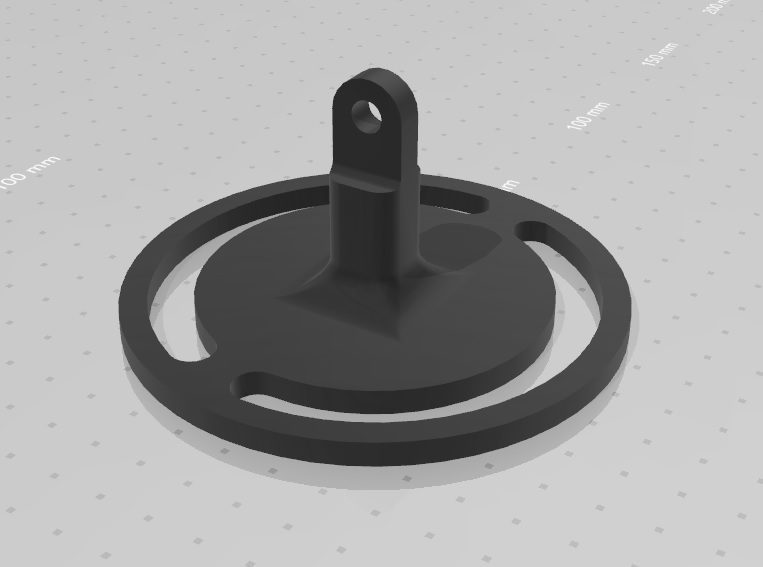
\includegraphics[scale=0.45]{images/halter.jpg}			
	\caption{camera fixture design.}
	\label{fig:camfix}                      
\end{figure}

To mount the cameras, item profiles \cite{Item} were used to build a simple structure to position the cameras.

It was not possible to monitor the whole workspace with only two cameras, so only one side of the robot workspace is monitored. The cameras were placed diagonally over the table which is placed inside the workspace as shown in Figure  \ref{fig:campos}.

\begin{figure}[H]                                      
	\centering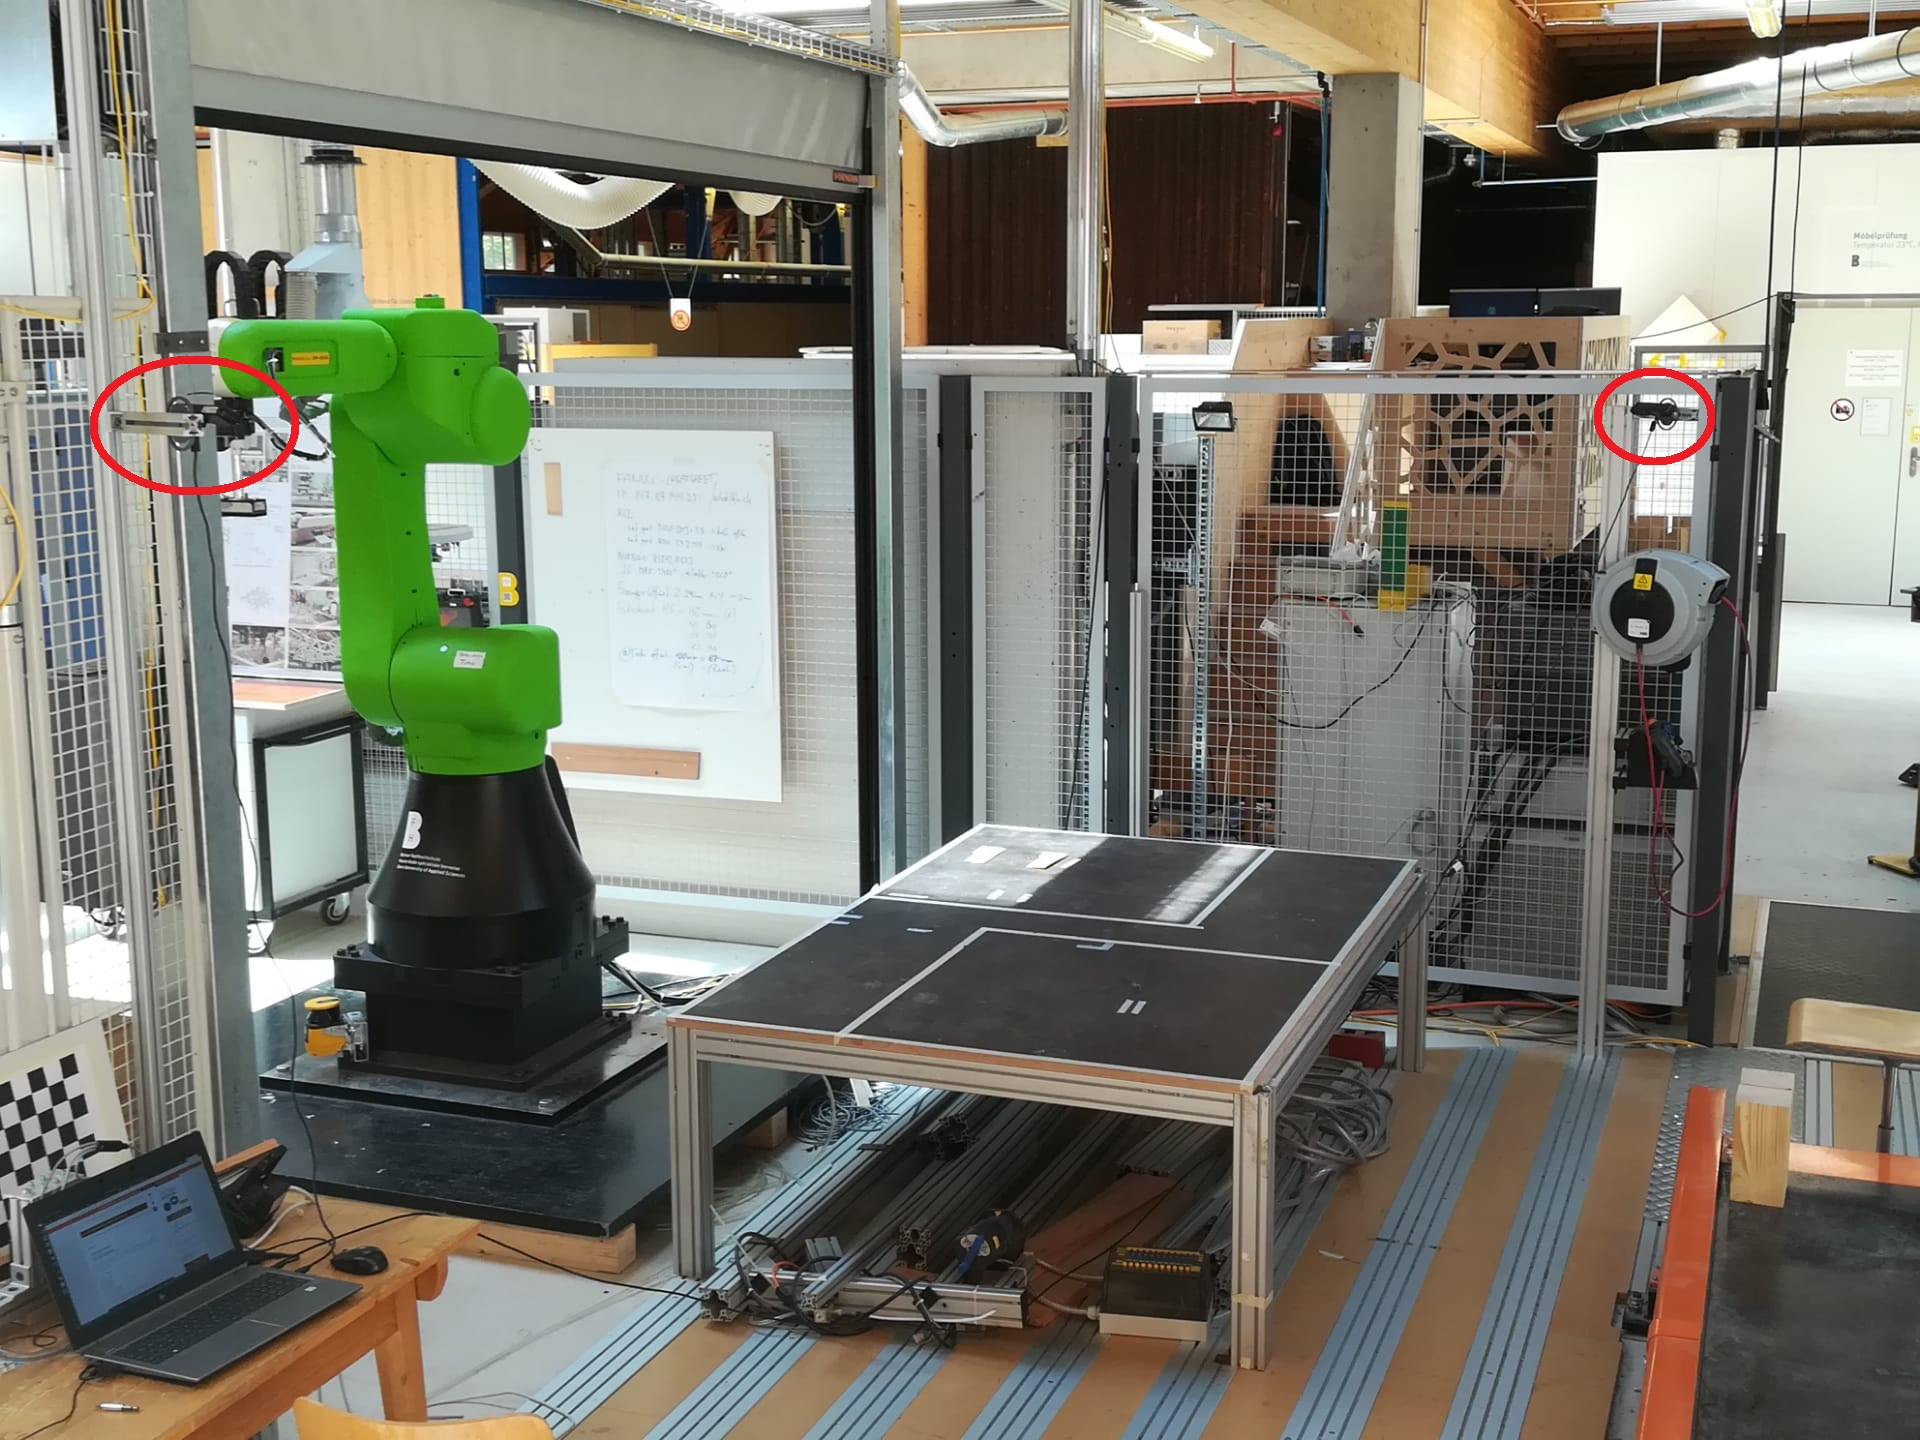
\includegraphics[scale=0.2]{images/campos.jpeg}			
	\caption{Final camera positions, cameras are marked red.}
	\label{fig:campos}                      
\end{figure}
 The diagonal positioning was chosen in order to have any side of objects on the table visible in the camera view. In a first approach the cameras were set up right beside the table, but since the projected infrared pattern of each camera interferes with each other, the cameras were moved further away from each other to reduce the intensity\cite{cameraInterference} of the infrared structure and thus to reduce the interference.

The interference of the cameras resulted in loss of data, but only on horizontal surfaces. The sides of the objects were still recognised, since each side of the object is only visible by a certain camera. Figure \ref{fig:infrared} shows the infrared pattern and how it behaves with obstacles in it.

%http://www.robotics.tu-berlin.de/fileadmin/fg170/Publikationen_pdf/martinmartin_14_ki_iros.pdf

\begin{figure}[H]                                      
	\centering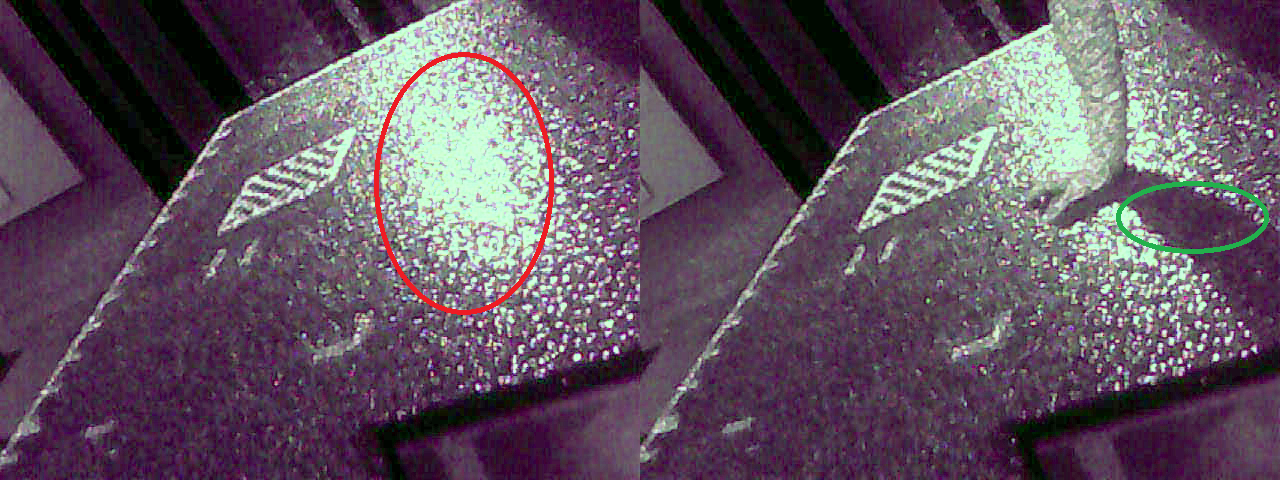
\includegraphics[scale=0.5]{images/Infrared.png}			
	\caption{Infrared structure capture. On the left side the interference, which results ins data loss, is marked in red. Green marked is the area which is inside the object shadow of one camera.}
	\label{fig:infrared}                      
\end{figure}

\subsection{Camera calibration}
\label{subsec:camcalib}
\lstset{language=C++,
	basicstyle=\ttfamily,
	keywordstyle=\color{blue},
	stringstyle=\color{red},
	commentstyle=\color{green},
	morecomment=[l][\color{magenta}]{\#}
}
The calibration of the cameras is done using CloudCompare and its possibility to align multiple point clouds to each other. For this a reference point cloud of the table (Figure \ref{fig:refpctable}) is generated when executing the camCalibration program. The program creates a point cloud with the surface of the table in red color. The two marked squares on the table are marked blue in the point cloud. For axis recognition a small green surface is created below the table (negative Z-direction). The table reference cloud is created at the position in the world frame of the robot.

\begin{figure}[H]                                      
	\centering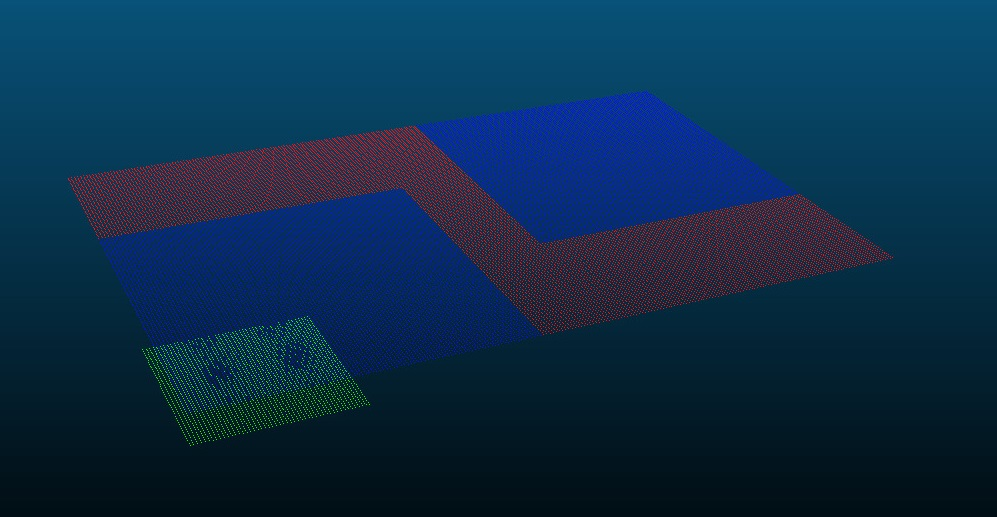
\includegraphics[scale=0.5]{images/CC_tableref.jpeg}			
	\caption{Reference point cloud of the table surface}
	\label{fig:refpctable}                      
\end{figure}

In addition a point cloud capture of the robot workspace from each camera is generated when the program is executed. The calibration is then done by loading the three point clouds into Cloud Compare and using the "Align two point clouds by picking (at least 4) equivalent points" command, which is located at in the top bar of Cloud Compare as marked with a red circle in figure \ref{fig:showpoints}. After clicking on the command button, a window appears in which the reference cloud can be set. Be sure to select the table reference cloud as reference.

\begin{figure}[H]                                      
	\centering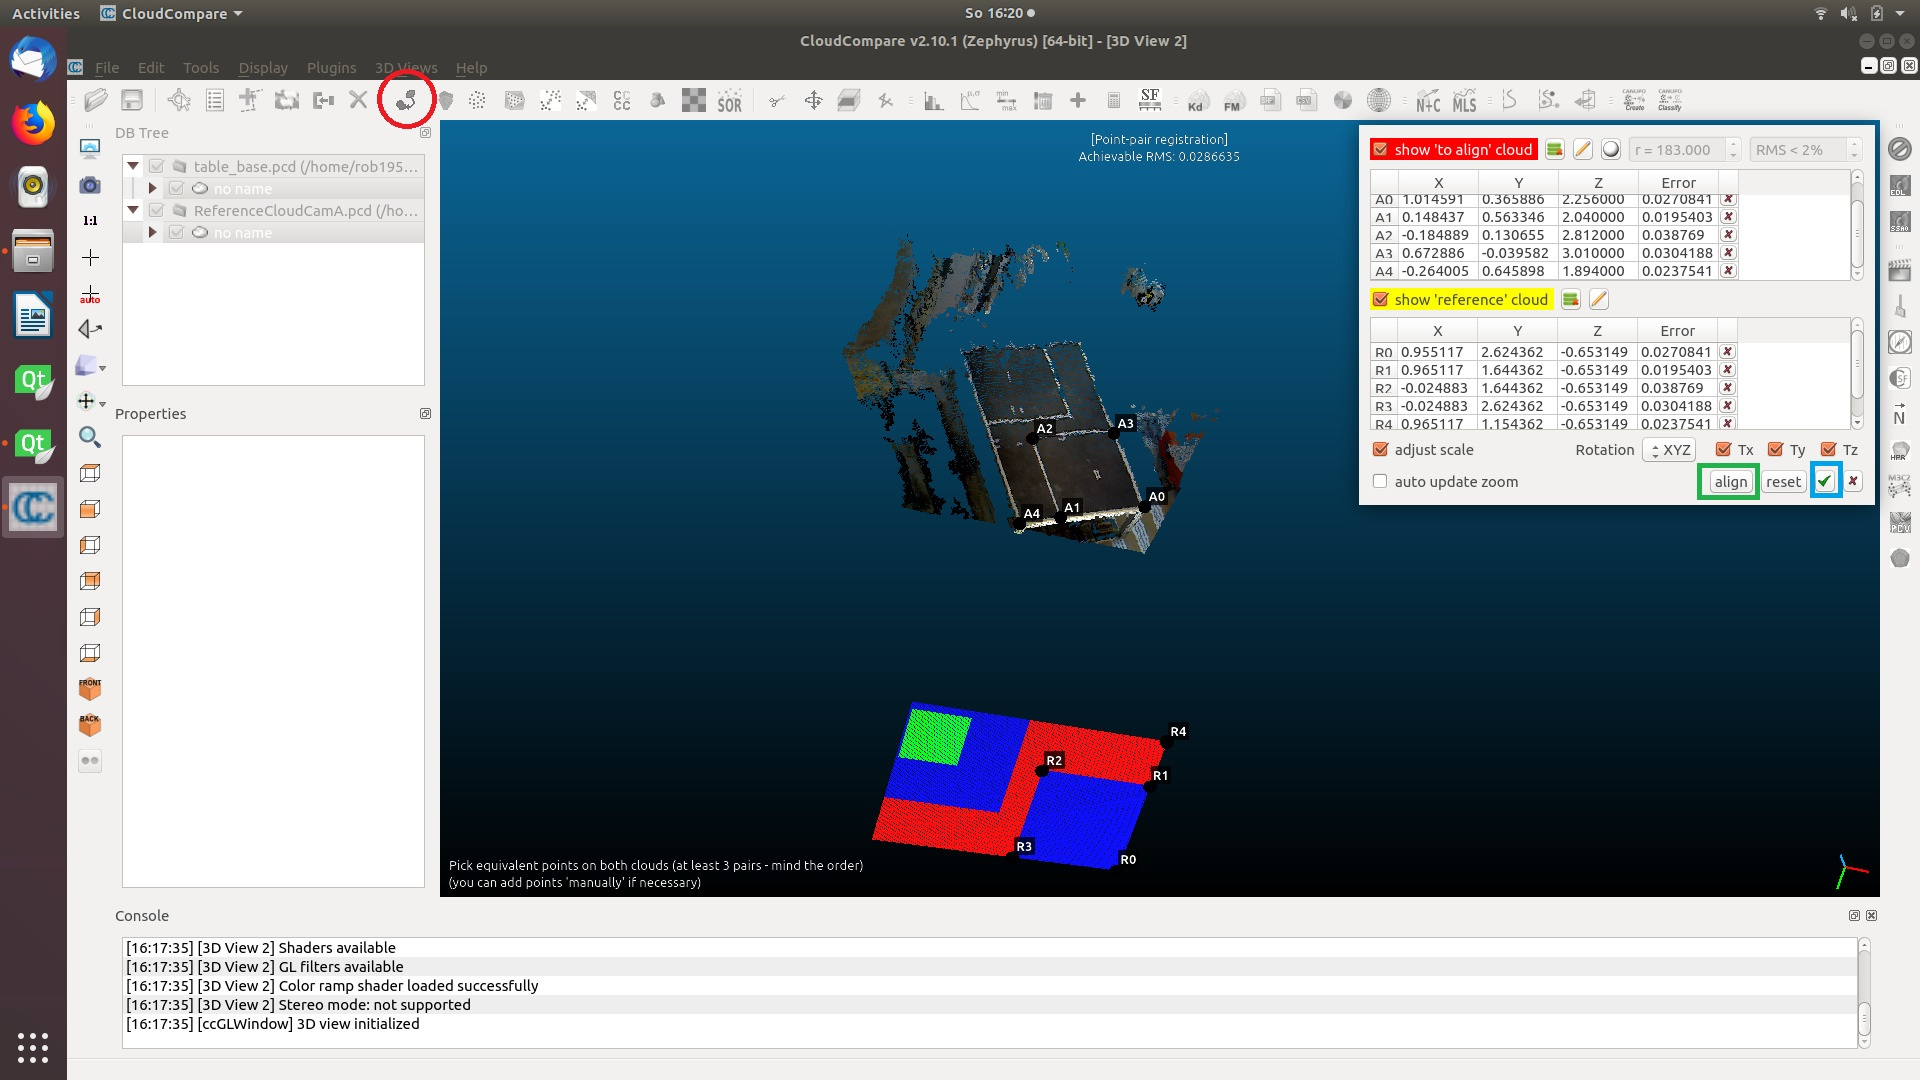
\includegraphics[scale=0.28]{images/CC_show_points.jpeg}			
	\caption{Table reference point cloud and a single camera generated poit cloud. Red Mark shows the "align" command. After picking the points the green marked "align" button can be clicked to show the result of the command. By clicking on the blue marked "approve" button, the changes are applied.}
	\label{fig:showpoints}                      
\end{figure}

\begin{figure}[H]                                      
	\centering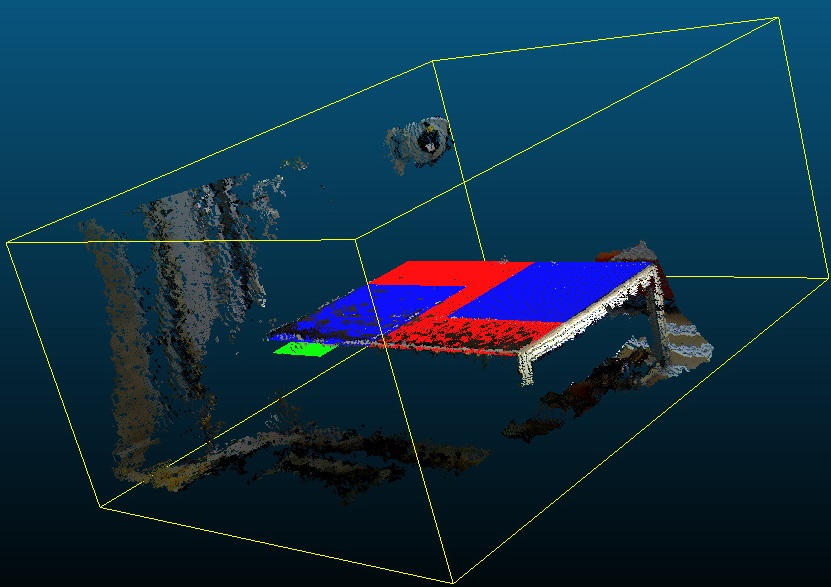
\includegraphics[scale=0.5]{images/CC_aligned_cloud.jpeg}			
	\caption{Single camera generated point cloud aligned with the table reference cloud.}
	\label{fig:cloudaligned}                      
\end{figure}

Figure \ref{fig:cloudaligned} shows a single point cloud aligned with the table reference. After aligning both camera generated point clouds, the transformation matrix can be found on the properties window, after selecting the specific point cloud, on the left side of Cloud Compare. This matrix can then be copied and pasted into the "cloudA.txt" respectively the "cloudB.txt" file, located in the Software/Rob195 folder. The matrices are then read into the collision avoidance software at the start of the main function (listing \ref{lst:matrixread}).
\begin{figure}[H]
\begin{lstlisting}[frame = single, caption={part of the main function of the collision avoidance system which reads the transformation matrices for camera A and B.}, captionpos=b, label={lst:matrixread}]  
// read cloud transformation data from file
ifstream fin ("./../Rob195/cloudA.txt");

if (fin.is_open()){
	for (int row = 0; row < nrows; row++){
		for (int col = 0; col < ncols; col++){
			float item = 0.0;
			fin >> item;
			transformCamA(row, col) = item;
		}
	}	
	fin.close();
}
ifstream fin2 ("./../Rob195/cloudB.txt");
if (fi2n.is_open()){
	for (int row = 0; row < nrows; row++){
		for (int col = 0; col < ncols; col++){
			float item = 0.0;
			fin2 >> item;
			transformCamB(row, col) = item;
		}
	}
	fin2.close();
}
\end{lstlisting}
\end{figure}
\subsection{Data acquisition}
\label{subsec:dataacq}

For the data acquisition the cameras were run using the OpenNI Grabber Framework in PCL. The simple openNI viewer class is available from the tutorials of the PCL. The example file was used and adapted to support a second camera. The \emph{run()} method of the class, creates for each camera a new OpenNIGrabber interface (listing \ref{lst:interface}). 
\lstset{language=C++,
	numbers=left,
	stepnumber=1,
	keywordstyle=\color{blue},
	stringstyle=\color{red},
	commentstyle=\color{green},
	morecomment=[l][\color{magenta}]{\#}
}
\begin{figure}[H]
\begin{lstlisting}[frame = single, caption={part of the run() function of the simple openNI viewer class}, captionpos=b, label={lst:interface}]  
 void run (){
	//**********************************
	//        start first Xtion
	Grabber* interface = new io::OpenNI2Grabber("#1");

	boost::function<void (const pcl::PointCloud
		<pcl::PointXYZRGBA>::ConstPtr&)> f =
	boost::bind (&SimpleOpenNIViewer::cloud_cb_, this, _1);

	interface->registerCallback (f);
	interface->start();
	//**********************************
	//**********************************
	//        start second Xtion
	pcl::Grabber* interface2 = new io::OpenNI2Grabber("#2");
	boost::function<void (const pcl::PointCloud
		<pcl::PointXYZRGBA>::ConstPtr&)> f2 =
	boost::bind (&SimpleOpenNIViewer::cloud_cb_2_, this, _1);

	interface2->registerCallback (f2);
	interface2->start();
	//**********************************
\end{lstlisting}
\end{figure}
\emph{pcl::PointCloud<pcl::PointXYZRGBA>::ConstPtr \&cloud} defines a pointer to a point cloud with color values (listing \ref{lst:callbackdef}). \emph{pcl::PointXYZ} would define a point cloud without color values. 
\begin{figure}[H]
\begin{lstlisting}[frame = single, caption={Function definition of the callback function, using a pointer to a point cloud with color values.}, captionpos=b, label={lst:callbackdef}]  
void cloud_cb_ (const pcl::PointCloud
	<pcl::PointXYZRGBA>::ConstPtr &cloud)
\end{lstlisting}
\end{figure}
The callback methods \emph{cloud\_cb\_()} and \emph{cloud\_cb\_2\_()} create at first a range filter to remove data which is out of bounds. This is realised with the \emph{pcl::PassThrough} object as shown in listing \ref{lst:passfilter}. The passthrough filter can be set up to specify in which axis the data needs to be filtered and at what range the data should be filtered. Be aware that for the set up of the filter the camera frame is used and the units used are meters. \emph{pass.setFilterLimitsNegative (true)} could be used to inverse the filter.
\begin{figure}[H]
\begin{lstlisting}[frame = single, caption={Passthrough filter for the camera input, to remove data which is out of bounds.}, captionpos=b, label={lst:passfilter}]  
pcl::PointCloud<pcl::PointXYZRGBA>::Ptr 
  CloudCamAfiltered (new pcl::PointCloud<pcl::PointXYZRGBA> ()); 
 // filter element
pcl::PassThrough<pcl::PointXYZRGBA> pass; 
pass.setInputCloud (cloud);
// axis definition
pass.setFilterFieldName ("z");	
// range definition, points from start to endpoint are included	
// in the pointcloud, the rest is filtered out.
pass.setFilterLimits (0.0, 4.1);

// pass.setFilterLimitsNegative (true);

// output cloud
pass.filter (*CloudCamAfiltered); 	
\end{lstlisting}
\end{figure}
After filtering out points out of bounds, the point clouds are downsampled using a voxelgrid filter element. This implements the octree data structure. The octree is a tree data structure in which each internal node has exactly eight children. The root node describes a cubic bounding box which encapsulates all points from the point cloud. By dividing this cube into eight smaller cubes, each representing a certain part of the root cube, the next level of the octree is generated as shown in figure \ref{fig:octree}. The node is always the center point of the cube it is representing. Processing a point cloud into an octree data structure already provides a form of voxelizing. The resolution can be chosen by defining how many layers the octree data structure should have or by defining the size of the cubes at the lowest level of the octree. 

\begin{figure}[H]                                      
	\centering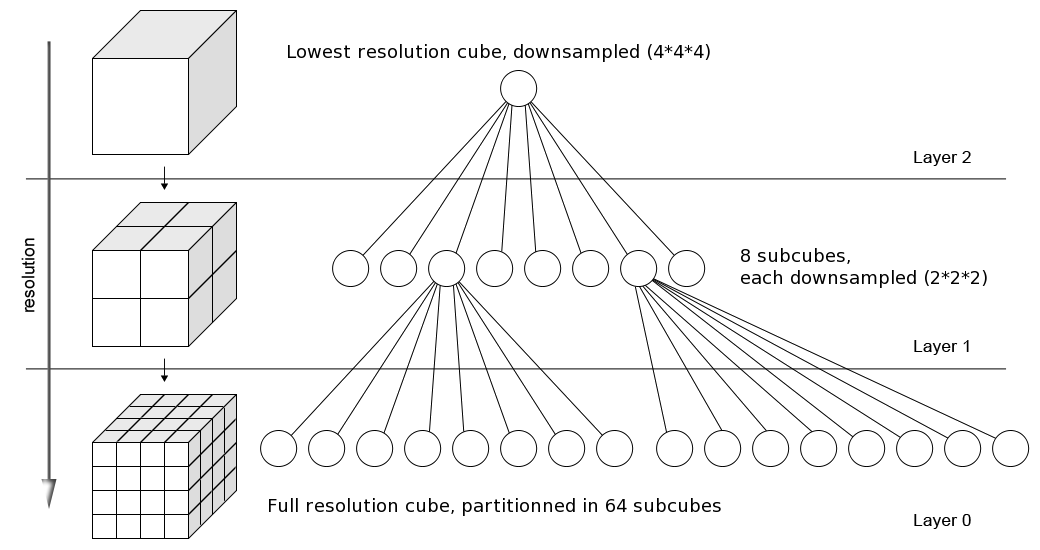
\includegraphics[scale=0.4]{images/Octree.png}			
	\caption{Graphical Illustration of an octree data structure}
	\label{fig:octree}                      
\end{figure}
\begin{figure}[H]
\begin{lstlisting}[frame = single, caption={Voxelgrid filter to downsample the point cloud and reduce the total amount of points.}, captionpos=b, label={lst:voxelfilter}]  
pcl::PointCloud<pcl::PointXYZRGBA>::Ptr 
   CloudCamAVoxelGrid (new pcl::PointCloud<pcl::PointXYZRGBA> ()); 
// filter element
pcl::VoxelGrid<pcl::PointXYZRGBA> voxelFilter; 
voxelFilter.setInputCloud(CloudCamAfiltered);
// cube size definition in meters
voxelFilter.setLeafSize (0.01f, 0.01f, 0.01f); 
// output cloud
voxelFilter.filter (*CloudCamAVoxelGrid); 
\end{lstlisting}
\end{figure}
After filtering, the point clouds are transformed to their exact position by using the previously generated transform matrices. This is done by using the \emph{pcl::transformPointCloud (*CloudCamAVoxelGrid, *transformedCloudCamA, transformCamA);} command. As parameters the input cloud, the output cloud and the transformation matrix have to be given to the function.

After transformation the point clouds are saved to the disk, when the program is executed with the debug flag (-d).

\section{Data processing and mapping}
\label{sec:process}
After the point clouds are pre-filtered and transformed into the necessary frame, a single point cloud is generated by concatenating (listing \ref{lst:concatenate}) the data from camera A and B. This is done inside the \emph{run()} function of the simpleOpenNIviewer class.
\begin{figure}[H]
\begin{lstlisting}[frame = single, caption={merging the point clouds from camera A and B into a single point cloud by concatenating the data.}, captionpos=b, label={lst:concatenate}]
*concatenatedCloud = *transformedCloudCamA;
*concatenatedCloud += *transformedCloudCamB;
\end{lstlisting} 
\end{figure}
The merged point cloud is then filtered again into the actual desired size of the cubes for the occupancy grid. The reason the merged point cloud is filtered again is simply due to avoid having data points close to each other by merging the point clouds from camera A and B. Since both cameras capture the same picture from a different angle, it is possible to have multiple points on the same spot. After applying the filter, an empty occupancy grid is created and afterwards filled with the data points from the merged point cloud. For this project a leaf size of 0.04m has been chosen since bigger leaf sizes appeared too big and inaccurate while lower leaf sizes resulted in longer calculating time. Figure \ref{fig:occupamcy} shows an occupancy grid created by the system.
\begin{figure}[H]
\begin{lstlisting}[frame = single, caption={Creating an empty occupancy grid of a specified leaf size. Then filling it with th point cloud data}, captionpos=b, label={lst:emptymap}]  
// creating map object and defining its leaf size
octomap::ColorOcTree tree( 0.04 ); 
for (float x = -2.5; x <= 2.5; x += 0.08f) { 
	for (float y = 0; y <= 4; y += 0.08f) {
		for (float z = -1.5; z <= 2; z += 0.08f) {
			octomap::point3d endpoint(x, y, z);
			// integrate 'free' measurement
			tree.updateNode(endpoint, false); 
		}
	}
}

//filling map with point cloud data
for (auto p:cloud_filtered->points){
	tree.updateNode(octomap::point3d(p.x, p.y, p.z), true);
}
// adding color information
for (auto p:cloud_filtered->points){
	tree.integrateNodeColor( p.x, p.y, p.z, p.r, p.g, p.b );
}
\end{lstlisting}
\end{figure}
\begin{figure}[H]                                      
	\centering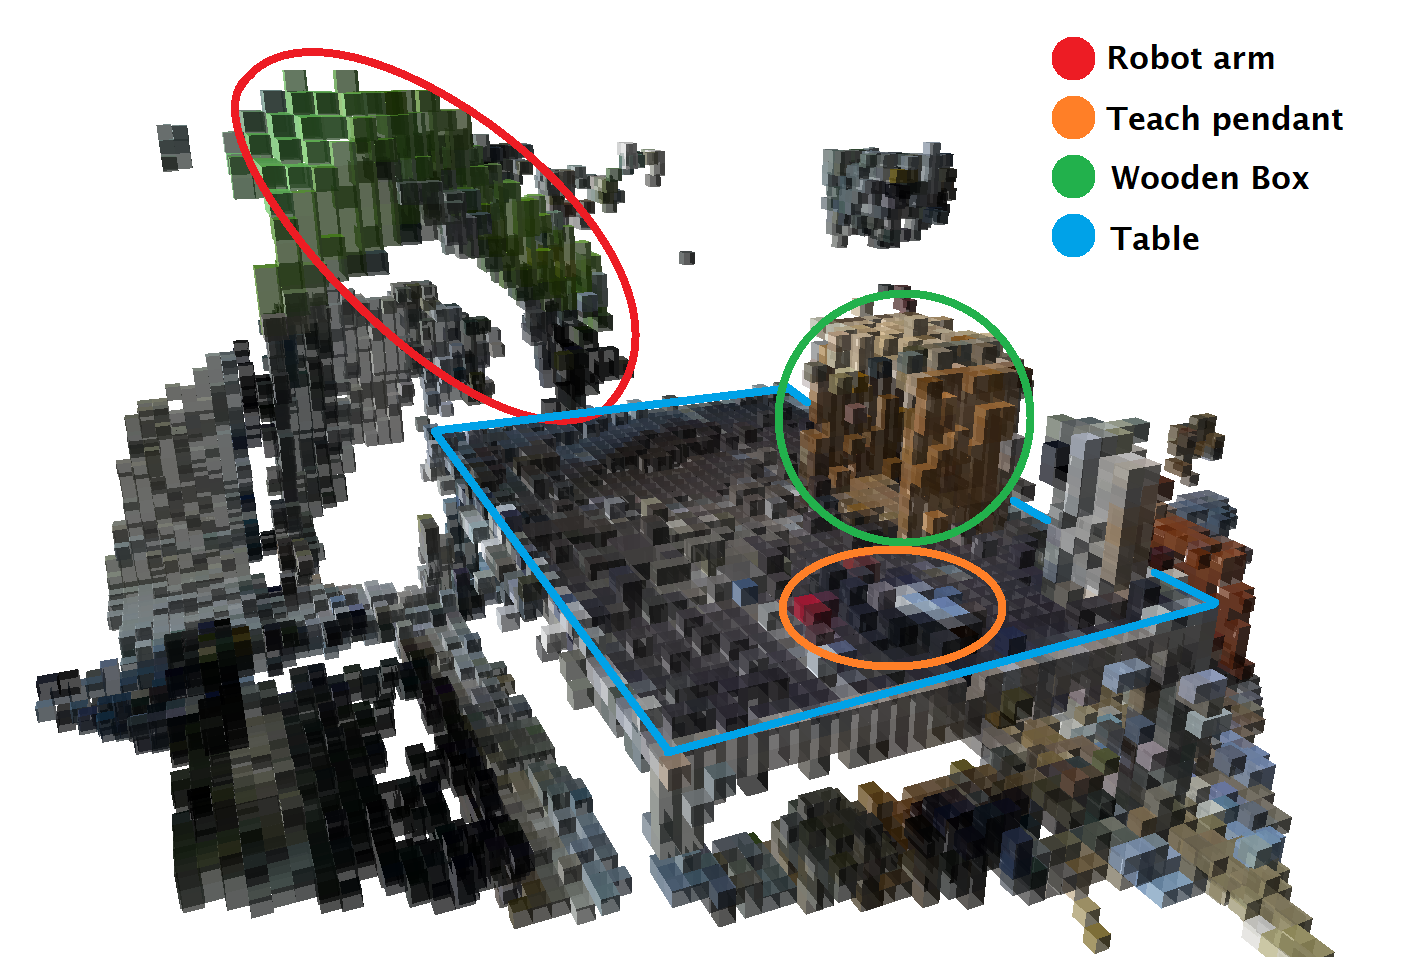
\includegraphics[scale=0.45]{images/occupancy_grid_marked.png}			
	\caption{Generated occupancy grid, already filled with the point cloud data.}
	\label{fig:occupamcy}                      
\end{figure}


\section{Collision avoidance}
\label{sec:avoid}

The collision avoidance also takes place in the \emph{run()} method of the viewer class. A while loop is executed as long as no safe and collision free path is found. Inside this while loop, a line is generated from the current robot position to the position where the robot should move to. The line is generated using the \emph{octomap::ColorOctree.castRay(point3d \&startingpoint, point3d \&direction, point3d \&endpoint, bool ignoreUknownCells, double maxRange )} function.
The starting point is received from the read robot position command. It is important to know that the current position read from the robot is received in millimeters, the unit used for the raycasting in the occupancy grid is meters. Be sure to have the correct units given to the \emph{octomap::ColorOctree.castRay()} function. The direction of the ray can be calculated with simple vector geometrics (\ref{eq:direction}).

\begin{equation}
\label{eq:direction}
	\begin{pmatrix}
	x_{goal}\\
	y_{goal}\\
	z_{goal}
	\end{pmatrix}
	-
	\begin{pmatrix}
	x_{current}\\
	y_{current}\\
	z_{current}
	\end{pmatrix}
	=
		\begin{pmatrix}
	x_{direction}\\
	y_{direction}\\
	z_{direction}
	\end{pmatrix}
\end{equation}

The endpoint returns the center coordinates of the first occupied cell that was hit by the ray. IgnoreUnknownCells defines how unknown cells are treated. For this project, unknown cells are treated as free cells and thus the value needs to be set to true. Since the point cloud data should cover all occupied cells, every other cell should be automatically set to free.
The distance the castRay has to cover can again easily be calculated with vector geometrics (\ref{eq:distance}).

\begin{equation}
\label{eq:distance}
	distance = \sqrt{(x_{goal}-x_{current})^2 + (y_{goal}-y_{current})^2 + (z_{goal}-z_{current})^2}
\end{equation}

The \emph{octomap::ColorOctree.castRay()} function returns a boolean, which is set to true if any occupied cell was hit and the maximum range was not reached. Therefore a true return values represents that an obstacle has been found. If an obstacle is found in the path of the robot, the robt moves a certain distance in z-Direction, in order to try to move over the object. After moving upwards, the castRay() starts again. To avoid reaching positions the robot can't reach, only a certain amount of increments along the z-Axis are done. After five attempts to avoid the obstacle, the program is paused and waits for a user input, approving that the object has been removed from the robot workspace.

Since the robot is captured by the cameras and therefore marked as occupied cells inside the map, any robot movement upwards  would generate a collision with the robot model. To avoid this straight upwards movements do not trigger a raycasting. The same goes for downwards movements when a piece should be picked up. The movement down to the piece would generate a collision with the piece and result in a collision. This means that for the use case created for this project only horizontal movements use the raycasting to detect collisions with objects in the robot workspace. Figure \ref{fig:system} shows a graphical overview on how the collision avoidance system operates.

\newpage
\begin{figure}[H]
	\centering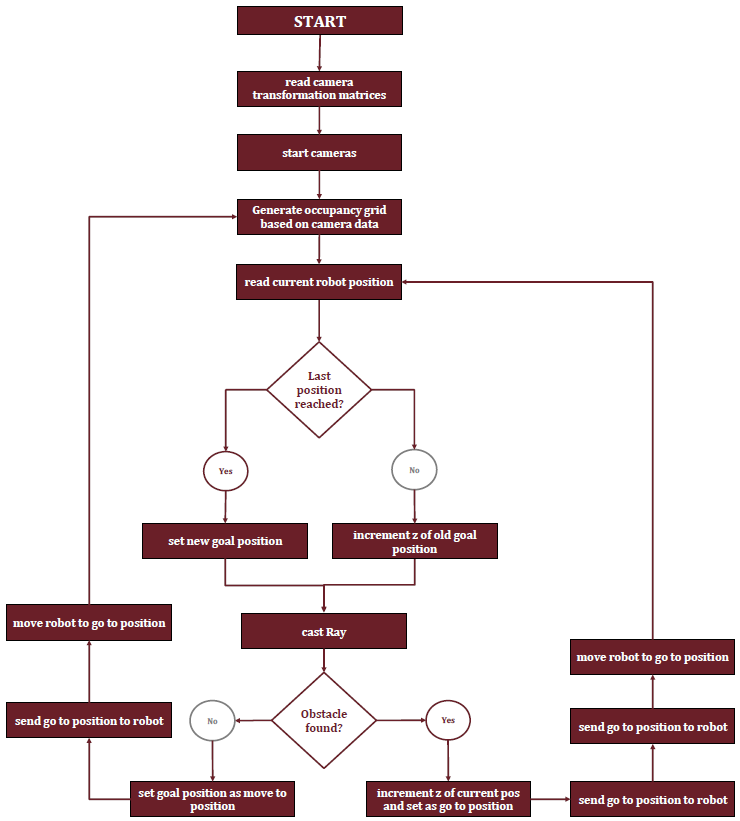
\includegraphics[scale=0.9]{images/system_overview.png}
	\caption{Graphical overview of the collision avoidance system.}
	\label{fig:system}
\end{figure}




